% !TEX root = ../main.tex
\chapter{Badania}
\label{ch:badania}

Rozdział ten został poświęcony szczegółowej prezentacji wyników ewaluacji czterech podejść do automatycznej detekcji nadużyć w komunikacji tekstowej użytkowników platformy C2C Stylify. Każde podejście zostało ocenione na tym samym zbiorze testowym, a~wyniki zostały przedstawione zarówno w formie tabelarycznej, jak i graficznej, umożliwiając bezpośrednie porównanie skuteczności i profilu błędów każdego z nich. Analiza wyników pozwoliła na sformułowanie wniosków dotyczących zalet i ograniczeń poszczególnych metod, a także na identyfikację obszarów wymagających dalszych badań i ulepszeń.

% ============================================================
\section{Metodyka ewaluacji}
\label{sec:metodyka}

Ewaluacja wszystkich czterech podejść przeprowadzona została
na~tym samym zbiorze testowym liczącym 120~przykładów, wyodrębnionym
ze~zbioru opisanego w~rozdziale~\ref{sec:dataset-podzial}.
Zbiór testowy był wyłączony z~procesu treningu i~doboru hiperparametrów;
jego skład był znany dopiero w~fazie końcowej ewaluacji, co~eliminuje
ryzyko wycieku danych (\english{data leakage}). Rozkład klas wynosi:
bypass~26, fraud~33, toxic~28, benign~33.

Dla każdego podejścia raportowane są następujące metryki klasyfikacji
wieloklasowej w~wariancie makro (nieważona średnia po~klasach):

\begin{equation}
  Precyzja ~(\english{Precision}) = \frac{1}{|C|}\sum_{c \in C} \frac{TP_c}{TP_c + FP_c},
  \label{eq:precision}
\end{equation}

\begin{equation}
  Pełność ~(\english{Recall}) = \frac{1}{|C|}\sum_{c \in C} \frac{TP_c}{TP_c + FN_c},
  \label{eq:recall}
\end{equation}

\begin{equation}
  Dokładność ~(\english{Accuracy}) = \frac{1}{N}\sum_{c \in C} TP_c,
  \label{eq:accuracy}
\end{equation}

\begin{equation}
  F_1 = \frac{1}{|C|}\sum_{c \in C} \frac{2 \cdot P_c \cdot R_c}{P_c + R_c},
  \label{eq:f1}
\end{equation}

\noindent gdzie $|C| = 4$, a~$TP_c$, $FP_c$, $FN_c$ oznaczają odpowiednio
liczbę prawdziwie pozytywnych, fałszywie pozytywnych i~fałszywie negatywnych
klasyfikacji dla~klasy~$c$. Dokładność (\english{accuracy}) definiowana jest
jako odsetek przykładów sklasyfikowanych poprawnie niezależnie od~klasy.

Błędy klasyfikacji podzielono na~trzy kategorie:
\begin{itemize}
  \item \textbf{FP} (\english{false positive}) - wiadomość klasy \textit{benign}
    zaklasyfikowana jako nadużycie (fałszywy alarm);
  \item \textbf{FN} (\english{false negative}) - nadużycie zaklasyfikowane
    jako \textit{benign} (pominięcie zagrożenia);
  \item \textbf{zła klasa} - nadużycie wykryte, lecz przypisane do~błędnej
    kategorii (np.\ bypass zamiast fraud).
\end{itemize}

% ============================================================
\section{Wyniki - Moduł~A: system regułowy}
\label{sec:wyniki-baseline}

% AUTO-GENEROWANY -- nie edytuj recznie!
% Zrodlo: experiments/evaluation/generate_figures.py

\begin{table}[H]
\centering
\caption{Metryki per klasa - Modul A (system regułowy)}
\label{tab:baseline-metrics}
\renewcommand{\arraystretch}{1.2}
\begin{tabular}{lrrrr}
\hline
\textbf{Klasa} & \textbf{Precyzja} & \textbf{Pełność} & \textbf{F\textsubscript{1}} & \textbf{N} \\
\hline
bypass & 0{,}419 & 0{,}500 & 0{,}456 & 26 \\
fraud & 1{,}000 & 0{,}182 & 0{,}308 & 33 \\
toxic & 0{,}000 & 0{,}000 & 0{,}000 & 28 \\
benign & 0{,}398 & 1{,}000 & 0{,}569 & 33 \\
\hline
\textbf{Makro} & 0{,}454 & 0{,}420 & 0{,}333 & 120 \\
\hline
\end{tabular}
\end{table}


System regułowy osiąga najsłabsze wyniki spośród wszystkich podejść:
makro~$F_1 = 0{,}333$, dokładność~$= 0{,}433$.
Wyniki dla każdej z klas (tabela~\ref{tab:baseline-metrics}) ujawniają strukturalną
słabość tego podejścia.

\paragraph{Klasa \textit{toxic} - F1 = 0{,}000.}
System regułowy nie zawiera żadnych reguł wykrywania toksyczności,
wszystkie 28~wiadomości klasy \textit{toxic} zaklasyfikowano jako \textit{benign}.
Jest to celowy wybór projektowy: system ten skupia się wyłącznie na~danych
kontaktowych i~frazach bypass, ignorując treści obraźliwe.
Konsekwencją jest zerowa pełność i~zerowa precyzja dla~tej klasy.

\paragraph{Klasa \textit{fraud} - F1 = 0{,}308.}
Mimo idealnej precyzji ($P = 1{,}000$), pełność wynosi tylko $R = 0{,}182$,
system wykrył jedynie 6~z~33 przypadków oszustwa.
Przyczyna leży w~kolejności reguł: wyrażenie regularne dla~numerów telefonów
jest sprawdzane \emph{przed} wzorcem IBAN, wskutek czego ciągi cyfr w~numerach
kont bankowych trafiają do~klasy \textit{bypass} zamiast \textit{fraud}.
Potwierdza to analiza błędów kategorii zła klasa (18 przypadków):
wiadomości zawierające numery IBAN lub kody BLIK systematycznie lądują
w~\textit{bypass}.

\paragraph{Klasa \textit{benign} - F1 = 0{,}569, R = 1{,}000.}
Idealna pełność dla~klasy neutralnej wynika z~tego, że~żadna wiadomość
\textit{benign} nie~jest błędnie flagowana jako nadużycie.
Jednocześnie wysoka liczba (50) pominiętych zagrożeń przekłada się na~zawyżoną
klasyfikację jako benign, stąd niska precyzja tej klasy ($P = 0{,}398$).

Podsumowując, system regułowy jest użyteczny jedynie jako szybki filtr danych
strukturalnych (e-mail, URL), nie zaś jako kompletne rozwiązanie.

% ============================================================
\section{Wyniki - Moduł~B: Presidio z~wyrażeniami regularnymi}
\label{sec:wyniki-presidio}

% AUTO-GENEROWANY -- nie edytuj recznie!
% Zrodlo: experiments/evaluation/generate_figures.py

\begin{table}[H]
\centering
\caption{Metryki per klasa - Modul B (Presidio + wyrazenia regularne)}
\label{tab:presidio-metrics}
\renewcommand{\arraystretch}{1.2}
\begin{tabular}{lrrrr}
\hline
\textbf{Klasa} & \textbf{Precyzja} & \textbf{Pełność} & \textbf{F\textsubscript{1}} & \textbf{N} \\
\hline
bypass & 1{,}000 & 0{,}962 & 0{,}980 & 26 \\
fraud & 1{,}000 & 1{,}000 & 1{,}000 & 33 \\
toxic & 1{,}000 & 0{,}857 & 0{,}923 & 28 \\
benign & 0{,}868 & 1{,}000 & 0{,}930 & 33 \\
\hline
\textbf{Makro} & 0{,}967 & 0{,}955 & 0{,}958 & 120 \\
\hline
\end{tabular}
\end{table}


Moduł~B osiąga makro~$F_1 = 0{,}958$, dokładność~$= 0{,}958$,
skok o~$+0{,}625$ względem Modułu~A ($+187{,}6\,\%$).
Precyzja wynosi $P = 1{,}000$ dla~klas bypass, fraud i~toxic
(tabela~\ref{tab:presidio-metrics}): każda wiadomość, którą Presidio
oznaczy jako nadużycie, jest nim rzeczywiście.

\paragraph{Klasa \textit{fraud} - F1 = 1{,}000.}
Kompletne pokrycie klasy fraud wynika z~bogactwa wzorców:
IBAN z~prawidłowym formatem, kody BLIK w~kontekście słów takich jak
,,blik'' czy ,,kod'', frazy zaliczkowe (,,wpłać z~góry'', ,,zadatek''),
linki phishingowe oraz prośby o~numer karty kredytowej.

\paragraph{Klasa \textit{toxic} - F1 = 0{,}923.}
Presidio wykrywa toksyczność poprzez słownik wulgaryzmów z~obsługą polskich
odmian (,,idiota-'', ,,kretyn'', ,,złodziej'' itp.) oraz frazy groźby.
Pozostałe 4~pominięte zagrożenia to wiadomości agresywne bez wulgaryzmów:
\textit{,,Tracę czas na takich jak ty!''},
\textit{,,Nie odpisujesz?! ODPOWIEDZ NATYCHMIAST!'},
\textit{,,Jesteś nikim do robienia interesów!''},
ton agresji wyrażony jest tu~przez kontekst i~interpunkcję, nie przez słowa kluczowe.

\paragraph{Klasa \textit{bypass} - 1 pominięte zagrożenie.}
Jedyna pominięta wiadomość bypass to:
\textit{,,Piszemy prywatnie, tu za dużo ludzi widzi daj znać''},
fraza semantyczna nieobecna w~słowniku wzorców bypass.

Moduł~B wykazuje zero błędów kategorii zła klasa: każde wykryte
nadużycie trafia do~właściwej klasy, co~potwierdza poprawność hierarchii
decyzyjnej (IBAN przed telefonem, zaliczki przed social media).

% ============================================================
\section{Wyniki - Moduł~C: Dostrojony HerBERT}
\label{sec:wyniki-herbert}

% AUTO-GENEROWANY -- nie edytuj recznie!
% Zrodlo: experiments/evaluation/generate_figures.py

\begin{table}[H]
\centering
\caption{Metryki per klasa - Modul C (dostrojony HerBERT)}
\label{tab:herbert-metrics}
\renewcommand{\arraystretch}{1.2}
\begin{tabular}{lrrrr}
\hline
\textbf{Klasa} & \textbf{Precyzja} & \textbf{Pełność} & \textbf{F\textsubscript{1}} & \textbf{N} \\
\hline
bypass & 0{,}929 & 1{,}000 & 0{,}963 & 26 \\
fraud & 1{,}000 & 0{,}970 & 0{,}985 & 33 \\
toxic & 1{,}000 & 1{,}000 & 1{,}000 & 28 \\
benign & 1{,}000 & 0{,}970 & 0{,}985 & 33 \\
\hline
\textbf{Makro} & 0{,}982 & 0{,}985 & 0{,}983 & 120 \\
\hline
\end{tabular}
\end{table}


Moduł~C osiąga makro~$F_1 = 0{,}983$, dokładność~$= 0{,}983$.
Jest to~wynik wyższy od~Modułu~B o~$+0{,}025$, przy~diametralnie
różnym profilu błędów (tabela~\ref{tab:herbert-metrics}).

\paragraph{Klasa \textit{toxic} - F1 = 1{,}000.}
HerBERT jako jedyne podejście osiąga perfekcyjne wyniki dla~toksyczności.
Model nauczył się rozpoznawać agresję semantyczną, wiadomości bez wulgaryzmów,
lecz wyrażające złość przez ton i~kontekst, czego nie był w~stanie zrobić
Moduł~B oparty na~słowniku.

\paragraph{Klasa \textit{bypass} - F1 = 0{,}963.}
Jedyny błąd to~1~przypadek fałszywego alarmu: wiadomość \textit{,,OK, dogadajmy szczegóły
wysyłki''} sklasyfikowana jako \textit{bypass}. Fraza ,,dogadajmy'' semantycznie
przypomina wyrażenia obejścia platformy (,,dogadajmy się poza serwisem''),
co~tłumaczy pomyłkę modelu. Ten~sam fałszywy alarm pojawia się we~wszystkich podejściach
opartych na~HerBERT (C i~D).

\paragraph{Klasa \textit{fraud} - 1 błąd kategorii.}
Jedna wiadomość klasy \textit{fraud} (prośba o~przelew) zaklasyfikowana
jako \textit{bypass}, model prawdopodobnie skojarzył frazy przelewowe
z~danymi kontaktowymi.

Łącznie Moduł~C popełnia 3~błędy na~120 przykładach (FP=1, FN=0, zła klasa=2).

% ============================================================
\section{Wyniki - Moduł~D: potok hybrydowy}
\label{sec:wyniki-hybrid}

% AUTO-GENEROWANY -- nie edytuj recznie!
% Zrodlo: experiments/evaluation/generate_figures.py

\begin{table}[H]
\centering
\caption{Metryki per klasa - Modul D (hybrydowy B+C)}
\label{tab:hybrid-metrics}
\renewcommand{\arraystretch}{1.2}
\begin{tabular}{lrrrr}
\hline
\textbf{Klasa} & \textbf{Precyzja} & \textbf{Pełność} & \textbf{F\textsubscript{1}} & \textbf{N} \\
\hline
bypass & 0{,}963 & 1{,}000 & 0{,}981 & 26 \\
fraud & 1{,}000 & 1{,}000 & 1{,}000 & 33 \\
toxic & 1{,}000 & 1{,}000 & 1{,}000 & 28 \\
benign & 1{,}000 & 0{,}970 & 0{,}985 & 33 \\
\hline
\textbf{Makro} & 0{,}991 & 0{,}992 & 0{,}991 & 120 \\
\hline
\end{tabular}
\end{table}


Moduł~D osiąga najwyższe wyniki spośród wszystkich podejść:
makro~$F_1 = 0{,}991$, dokładność~$= 0{,}992$.

\paragraph{Routing w~potoku.}
Na~120~wiadomości testowych Presidio (B) obsłużył
82 przypadki (68{,}3\,\%), a~HerBERT (C), 38~przypadków
(31{,}7\,\%) (rys.~\ref{fig:hybrid-routing}).
Oznacza to, że~ponad dwie trzecie wiadomości jest klasyfikowanych
przez szybki moduł B, bez konieczności uruchamiania modelu neuronowego.
Jest to~istotna zaleta dla~wydajności systemu produkcyjnego opisana poniżej.

\begin{figure}[H]
\centering
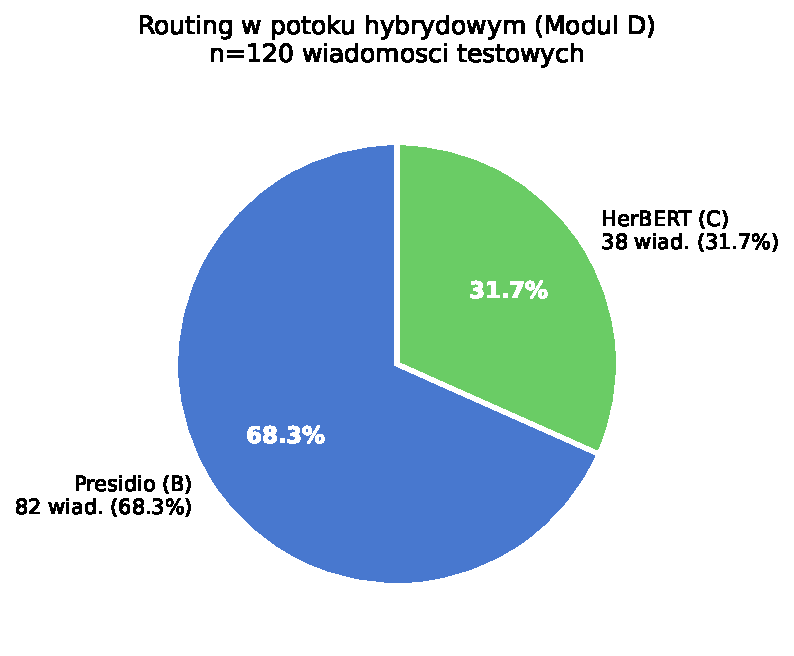
\includegraphics[width=0.55\textwidth]{chapters/figures/fig_hybrid_routing.pdf}
\caption{Routing wiadomości w~potoku hybrydowym , 68{,}3\,\% trafia
  do~Presidio, 31{,}7\,\% do~HerBERT}
\label{fig:hybrid-routing}
\end{figure}


\paragraph{Testy wydajności potoku.}

W celu weryfikacji założeń architektonicznych przeprowadzono pomiary czasów przetwarzania wiadomości dla poszczególnych komponentów systemu. Uzyskane wyniki jednoznacznie potwierdzają słuszność zastosowania potoku hybrydowego. Moduł B, oparty na bibliotece Presidio, charakteryzuje się średnim czasem odpowiedzi na poziomie 8,38 ms. Z kolei semantyczna klasyfikacja z wykorzystaniem modelu HerBERT (Moduł C) jest operacją znacznie bardziej kosztowną obliczeniowo, trwającą średnio 43,48 ms. Analiza wyższych percentyli (p95 oraz p99) dowodzi stabilności i przewidywalności obu rozwiązań, jednak ponad pięciokrotna różnica w szybkości działania uwydatnia główną zaletę Modułu D. Odfiltrowanie większości ruchu już na etapie lekkiego detektora wstępnego pozwala drastycznie zredukować sumaryczne obciążenie systemu, co jest kluczowe dla zachowania płynności komunikacji w czasie rzeczywistym.
\begin{table}[htbp]
\centering
\caption{Czasy przetwarzania wiadomości w potoku hybrydowym (Moduł D)}
\label{tab:wydajnosc_potoku}
\begin{tabular}{lcccc}
\toprule
\textbf{Pomiar} & \textbf{Liczba} & \textbf{Średnia} & \textbf{p95} & \textbf{p99} \\
\midrule
B - Presidio & 140 & 8,38 ms & 10,19 ms & 12,50 ms \\
C - HerBERT  & 60  & 43,48 ms & 54,86 ms & 76,14 ms \\
\bottomrule
\end{tabular}
\end{table}

\paragraph{Uzupełnianie błędów.}
Moduł~D eliminuje jedyny błąd kategorii Modułu~C: wiadomość \textit{fraud}
błędnie klasyfikowaną przez HerBERT jako \textit{bypass} jest teraz poprawnie
wykrywana przez Presidio (rozpoznaje IBAN/BLIK) na~pierwszym etapie potoku,
zanim HerBERT w~ogóle zostanie wywołany. W~efekcie $F_1(\text{fraud}) = 1{,}000$
przy~zachowaniu $F_1(\text{toxic}) = 1{,}000$ dziedziczonego z~Modułu~C.

Jedynym pozostałym błędem jest ten sam~fałszywy alarm co~w~Module~C: wiadomość
\textit{,,OK, dogadajmy szczegóły wysyłki''} zaklasyfikowana jako bypass.
Presidio nie~wykrywa jej jako nadużycia (brak wzorca), więc sprawa trafia
do~HerBERT, który popełnia tę~samą pomyłkę semantyczną.

% ============================================================
\section{Porównanie podejść}
\label{sec:porownanie}

\subsection{Zbiorcza tabela metryk}

Poniższa tabela~\ref{tab:comparison} zestawia wszystkie metryki dla~czterech podejść
w~jednym miejscu, umożliwiając bezpośrednie porównanie skuteczności i~profilu błędów każdego z~nich.

% AUTO-GENEROWANY -- nie edytuj recznie!
% Zrodlo: experiments/evaluation/generate_figures.py

\begin{table}[H]
\centering
\caption{Zbiorcze porownanie skutecznosci czterech podejsc}
\label{tab:comparison}
\renewcommand{\arraystretch}{1.2}
\begin{tabular}{lrrrr}
\hline
\textbf{Podejście} & \textbf{Precyzja} & \textbf{Pełność} & \textbf{F\textsubscript{1}} & \textbf{Dokładność} \\
\hline
System regułowy (A) & 0{,}454 & 0{,}420 & 0{,}333 & 0{,}433 \\
Presidio\ + wyrażenia regularne (B) & 0{,}967 & 0{,}955 & 0{,}958 & 0{,}958 \\
Dostrojony HerBERT\ (C) & 0{,}982 & 0{,}985 & 0{,}983 & 0{,}983 \\
Hybrydowy B+C (D) & 0{,}991 & 0{,}992 & 0{,}991 & 0{,}992 \\
\hline
\end{tabular}
\end{table}



\subsection{Wzrost skuteczności}

\begin{figure}[H]
\centering
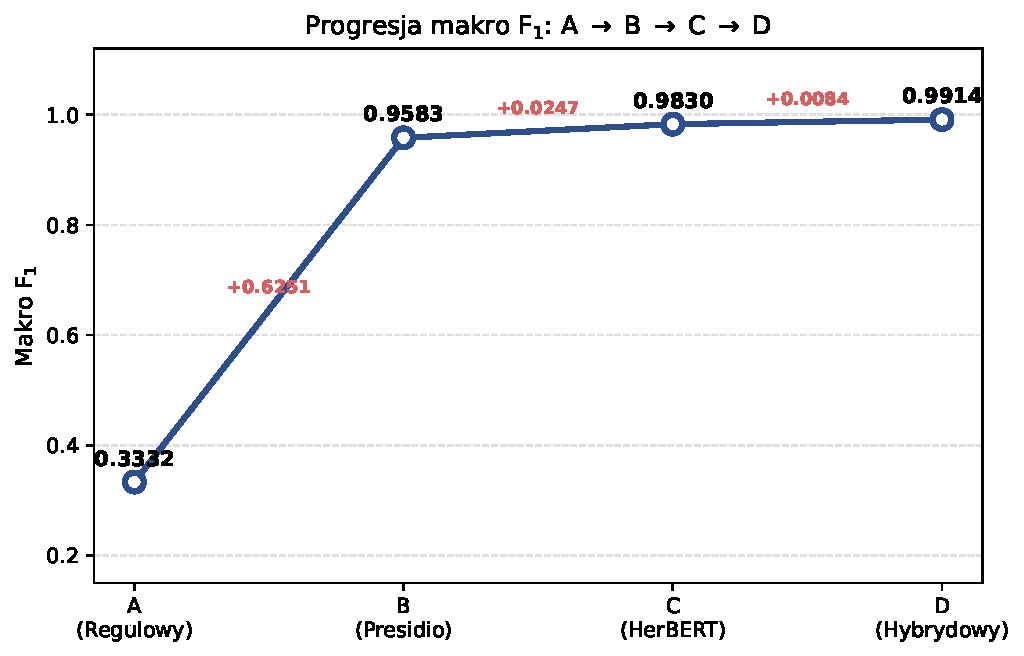
\includegraphics[width=0.80\textwidth]{chapters/figures/fig_f1_progression.pdf}
\caption{Wzrost makro~$F_1$ w~kolejności podejść A~$\to$~B~$\to$~C~$\to$~D}
\label{fig:f1-progression}
\end{figure}

Rysunek~\ref{fig:f1-progression} ilustruje wzrost makro~$F_1$.
Największy skok następuje między~A i~B ($+0{,}625$), przejście od~trywialnych
wyrażeń regularnych do~rozbudowanego systemu Presidio który lepiej wyłapuje kontekst.
Kolejne przyrosty (B$\to$C: $+0{,}025$; C$\to$D: $+0{,}008$) są~mniejsze,
lecz jakościowo istotne: Moduł~C wnosi semantyczne rozumienie toksyczności,
a~Moduł~D naprawia błąd kategorii oszustw.

\subsection{Porównanie metryk szczegółowych}

\begin{figure}[H]
\centering
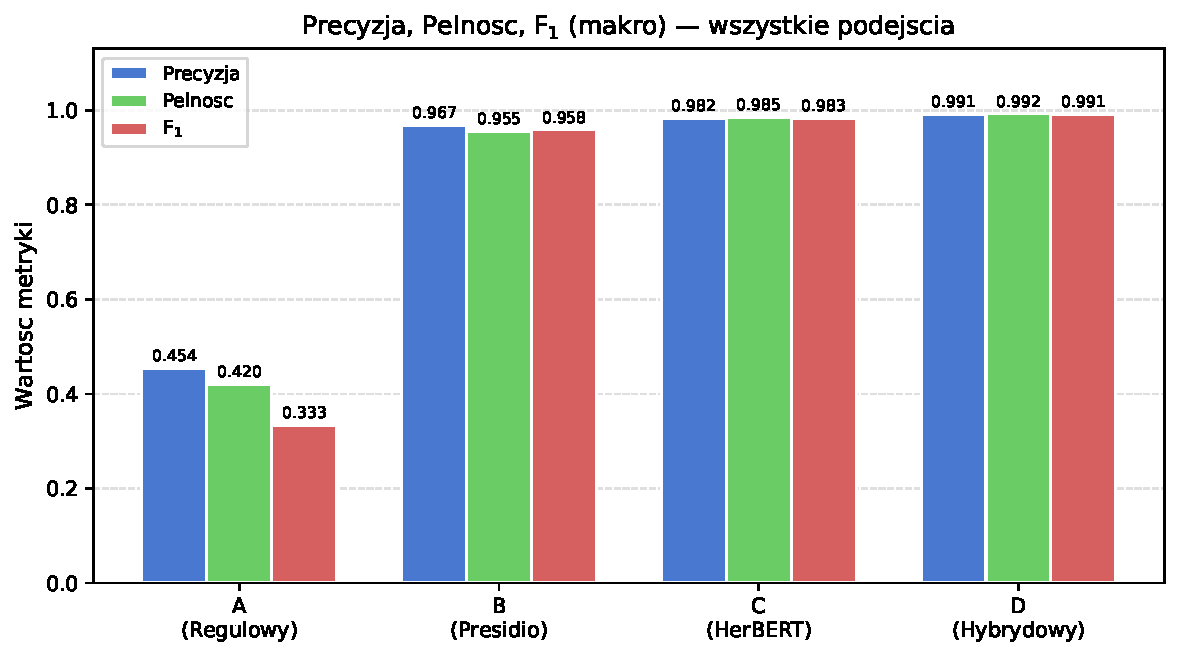
\includegraphics[width=0.85\textwidth]{chapters/figures/fig_prf_comparison.pdf}
\caption{Precyzja, pełność i~$F_1$ (makro) dla~wszystkich podejść}
\label{fig:prf-comparison}
\end{figure}

\begin{figure}[H]
\centering
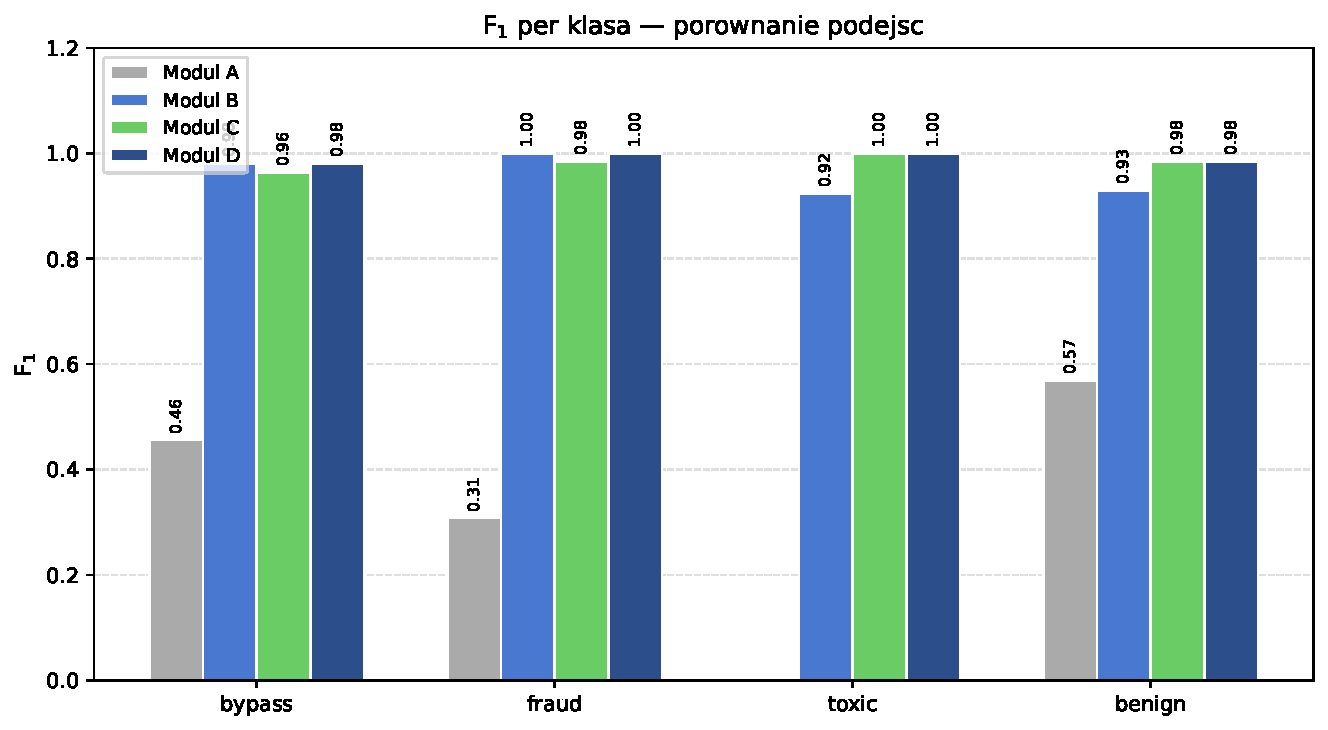
\includegraphics[width=0.85\textwidth]{chapters/figures/fig_per_class_f1.pdf}
\caption{Porównanie $F_1$ dla~poszczególnych klas}
\label{fig:per-class-f1}
\end{figure}

Detekcja danych osobowych za~pomocą Presidio radykalnie poprawia skuteczność
przy zerowych kosztach fałszywych alarmów. Moduł~B osiągnął makro~$F_1 = 0{,}958$,
wzrost o~$+187{,}6\,\%$ względem Modułu~A. Architektura Presidio eliminuje błędy kategorii (zero przypadków błędnej klasy), a~precyzja
dla~klas bypass, fraud i~benign wynosi $1{,}000$. Granicą tego podejścia są
wiadomości toksyczne wyrażone bez wulgaryzmów ze~słownika, 5 takich przypadków
pozostało nieoznaczonych.

Rysunek~\ref{fig:prf-comparison} pokazuje, że~Moduł~A cierpi przede wszystkim
na~niską pełność ($R = 0{,}420$), system nie~wykrywa nadużyć, nie~zaś
fałszywie je~sygnalizuje ($P = 0{,}454$, FP~=~0). Moduły B-D utrzymują
precyzję powyżej $0{,}963$.

Rysunek~\ref{fig:per-class-f1} uwidacznia kluczową różnicę między~B a~C:
\textit{toxic} rośnie z~$F_1 = 0{,}923$ (Moduł~B) do~$F_1 = 1{,}000$
(Moduł~C i~D). Dla~klas bypass i~fraud Presidio (B) osiąga wyniki porównywalne
lub wyższe od~samego HerBERT, co~uzasadnia jego rolę jako pierwszego
etapu w~potoku hybrydowym.

\subsection{Macierze pomyłek}

\begin{figure}[H]
\centering
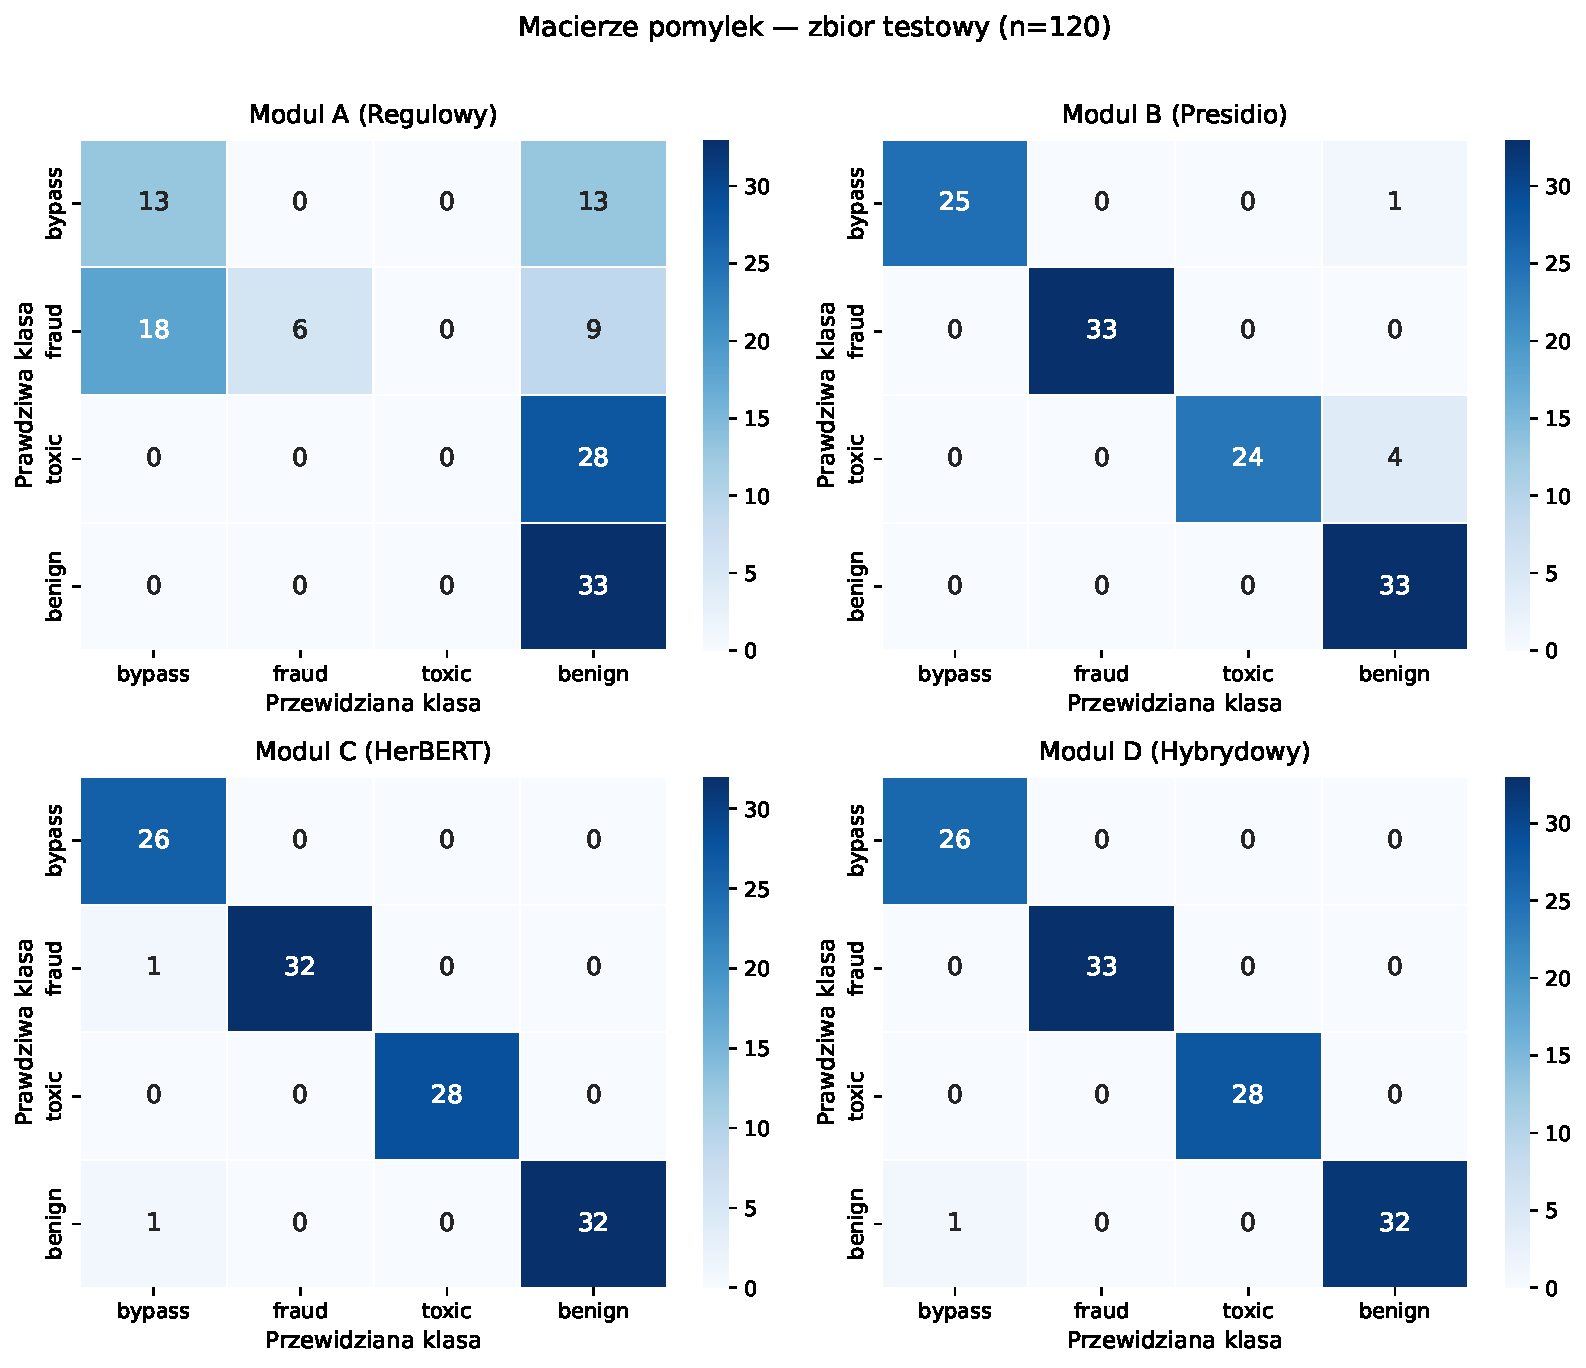
\includegraphics[width=\textwidth]{chapters/figures/fig_confusion_matrices.pdf}
\caption{Macierze pomyłek dla~wszystkich czterech podejść
  (wiersze = klasa prawdziwa, kolumny = klasa przewidziana)}
\label{fig:all-confusion-matrices}
\end{figure}

Rysunek~\ref{fig:all-confusion-matrices} zestawia macierze pomyłek.
W~Module~A widoczna jest całkowita nieobecność wykryć klasy toxic
oraz rozproszenie klasy fraud między bypass (18 przypadków) i~benign (9 przypadków).
Moduły B-D mają macierze bliskie diagonalnym, a~Moduł~D jest praktycznie
perfekcyjny, jedyna pomyłka to 1 przykład benign sklasyfikowany jako bypass.

% ============================================================
\section{Analiza błędów}
\label{sec:analiza-bledow}

\begin{figure}[H]
\centering
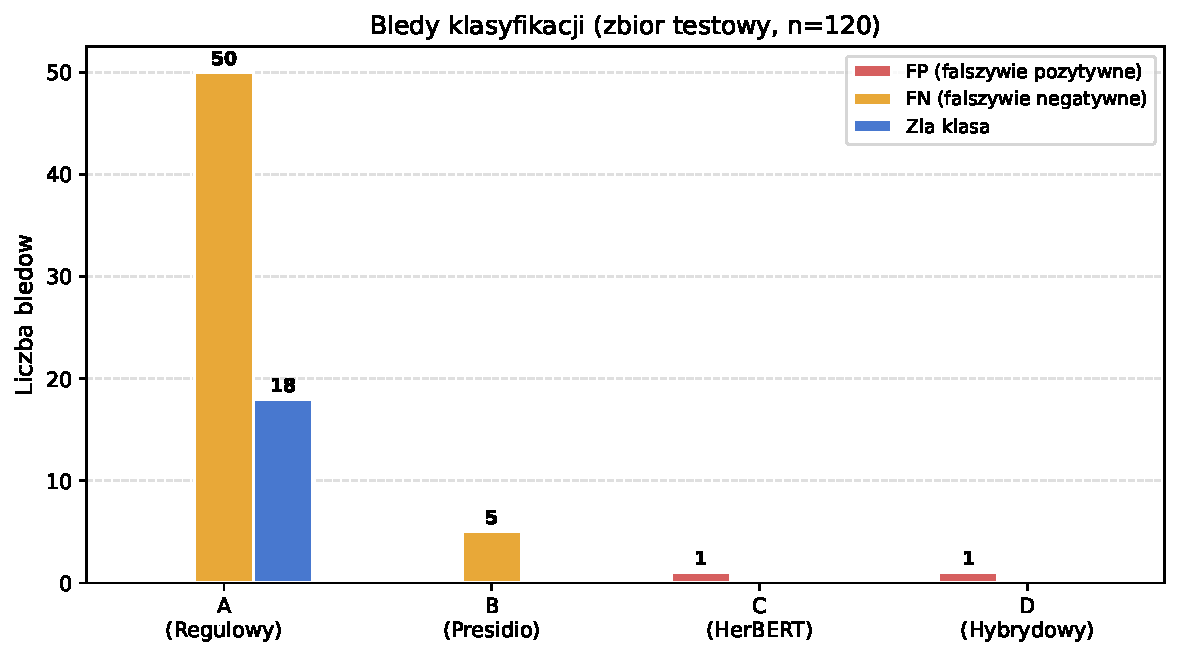
\includegraphics[width=0.82\textwidth]{chapters/figures/fig_error_analysis.pdf}
\caption{Liczba błędów klasyfikacji per podejście}
\label{fig:error-analysis}
\end{figure}

Rysunek~\ref{fig:error-analysis} przedstawia liczby fałszywych alarmów (FP), pominięte zagrożenia (FN) i~błędów kategorii
per podejście. Łączna liczba błędów spada z~68 (Moduł~A) do~5 (B), 2 (C) i~1 (D).

\subsection{Typowe błędy Modułu~A}

\textbf{Pominięte zagrożenia (FN = 50):}
\begin{itemize}
  \item \textit{,,Czekam tydzień i nic, ty idioto''} , toxic; brak reguły toksyczności.
  \item \textit{,,Dogadajmy się poza serwisem, będzie szybciej''} , bypass; fraza
    semantyczna nieobecna w~słowniku.
  \item \textit{,,Zapłać z góry to wysyłam tego samego dnia''} , fraud (zaliczka);
    brak wzorca zaliczkowego.
\end{itemize}

\textbf{Błędy kategorii (18 przypadków):}
Ciągi cyfr w~numerach IBAN i~kodach BLIK dopasowywane są przez \texttt{PHONE\_REGEX}
zamiast \texttt{IBAN\_REGEX}, wynik: fraud klasyfikowany jako bypass.
Przykład: \textit{,,Transfer na: PL7488059296... Sprawdź.''} $\to$ bypass (zamiast fraud).

\subsection{Typowe błędy Modułu~B}

\textbf{Pominięte zagrożenia (FN = 5), wszystkie w~klasie toxic:}
\begin{itemize}
  \item \textit{,,Tracę czas na takich jak ty!''} , brak wulgaryzmu; agresja wyrażona frustracją.
  \item \textit{,,Nie odpisujesz?! ODPOWIEDZ NATYCHMIAST!''} , agresja przez caps lock
    i~nadmiar wykrzykników; poza słownikiem toksyczności.
  \item \textit{,,Jesteś nikim do robienia interesów!!''} , obelga leksykalnie łagodna.
  \item \textit{,,Ostatni raz pytam zanim zgłoszę. Serio.''} , ukryta groźba bez słów
    kluczowych.
\end{itemize}

Wspólny mianownik: toksyczność semantyczna bez obecności wulgaryzmów ze~słownika.
Podejście oparte wyłącznie na~wzorcach nie~jest w~stanie jej uchwycić.

\subsection{Typowe błędy Modułów~C i~D}

\textbf{Jedyny fałszywy alarm (obie podejścia):}
\textit{,,OK, dogadajmy szczegóły wysyłki''} $\to$ bypass.
Fraza ,,dogadajmy'' jest leksykalnie bliska wyrażeniom obejścia platformy
(,,dogadajmy się poza serwisem''), a~wiadomość jest zbyt krótka, by~model
mógł rozróżnić kontekst transakcyjny od~nadużycia.
Jest to~przykład graniczny (\english{edge case}): fraza jest semantycznie
dwuznaczna i~mogłaby równie dobrze pojawić się w~rzeczywistym ataku bypass.

% ============================================================
\section{Odpowiedź na pytanie badawcze}
\label{sec:odpowiedz}

Pytanie badawcze sformułowane w~rozdziale~\ref{sec:pytanie} brzmi:
\textit{Które podejście najskuteczniej wykrywa nadużycia w~polskojęzycznym
czacie platformy marketplace przy jednoczesnym zachowaniu akceptowalnej
liczby fałszywych alarmów?}

\medskip
\noindent \textbf{Odpowiedź:} Najlepszym podejściem jest \textbf{Moduł~D}
(potok hybrydowy Presidio~+~HerBERT), który osiąga:

\begin{itemize}
  \item makro $F_1 = 0{,}991$ (wzrost o~$+197{,}5\,\%$ względem Modułu~A);
  \item dokładność $= 0{,}992$ , tylko 1 błąd na 120 wiadomości;
  \item $F_1 = 1{,}000$ dla klas \textit{fraud} i~\textit{toxic},
    najpoważniejsze kategorie nadużyć wykrywane bezbłędnie;
  \item zaledwie 1~fałszywy alarm na~120 przykładów, minimalne ryzyko blokady
    legalnych wiadomości.
\end{itemize}

\noindent Jednocześnie warto podkreślić, że:
\begin{itemize}
  \item \textbf{Moduł~C} (samo HerBERT, $F_1 = 0{,}983$) jest praktyczną
    alternatywą, gdy~uproszczenie stosu technologicznego jest priorytetem, różnica $F_1$ względem D wynosi tylko $0{,}008$.
  \item \textbf{Moduł~B} (samo Presidio, $F_1 = 0{,}958$) sprawdza się znakomicie
    dla~wzorców strukturalnych (numer telefonu, IBAN, BLIK, media społecznościowe)
    i~jest najszybszym podejściem obliczeniowo.
  \item \textbf{Moduł~A} (system regułowy, $F_1 = 0{,}333$) jest niewystarczający
    jako samodzielna obrona, jego rola to jedynie szybki filtr, który musi być ciągle aktualizowany, nie~zaś kompleksowe rozwiązanie do~detekcji nadużyć.
\end{itemize}

\noindent Wyniki jednoznacznie potwierdzają, że~podejście oparte
na~uczeniu maszynowym (dostrajanie polskiego modelu językowego HerBERT
\cite{bib:herbert}) znacząco przewyższa podejścia regułowe w~każdej
mierzonej metryce. Kluczowym wkładem potoku hybrydowego D jest połączenie
precyzji strukturalnej Presidio \cite{bib:presidio} z~semantycznym rozumieniem
HerBERT: dwie trzecie ruchu (68{,}3\,\%) obsługiwane jest przez szybki moduł~B
bez~wywołania modelu neuronowego, co~minimalizuje opóźnienie w~środowisku
produkcyjnym oraz minimalizuje koszty operacyjne co jest istotną zaletą.
